%%
%% CSD Assignment 1 - Add-on: OpenTelemetry in the Village Pond Planning System
%% Same course template as the final report (ACM "acmart", single-column manuscript).
%% Local build: `make report-otel` -> docs/report/OpenTelemetry_Report.pdf
%%
\documentclass[manuscript,screen,review]{acmart}

\AtBeginDocument{%
  \providecommand\BibTeX{{Bib\TeX}}}

\usepackage{tikz}
\usetikzlibrary{positioning,arrows.meta,fit,backgrounds}
\usepackage{tabularx}
\usepackage{listings}
\newcolumntype{L}{>{\raggedright\arraybackslash}X}
\lstset{basicstyle=\ttfamily\footnotesize,breaklines=true,columns=fullflexible,frame=single}

\newcommand{\repourl}{https://github.com/Rahul5977/CSD-Course/tree/main/Project/1.PondPlanning}

\begin{document}

\title{OpenTelemetry in the AI-based Village Pond Planning System}
\subtitle{CSD Assignment 1 -- Add-on: observability with traces, metrics and logs}

\author{Rahul Raj\protect\\ \protect\normalfont\protect\small Student ID: 12341680}
\affiliation{%
  \institution{Indian Institute of Technology Bhilai}
  \city{Bhilai}
  \country{India}}
\email{rahul.raj9237@gmail.com}
\renewcommand{\shortauthors}{Rahul Raj}

\begin{abstract}
We added OpenTelemetry (OTel) to the existing Village Pond Planning System (Assignment~1).
Every Python process --- the FastAPI service and the two Celery worker pools --- exports
traces, metrics and logs over OTLP to an OpenTelemetry Collector. The collector routes
traces to Jaeger, metrics to Prometheus and logs to Loki, and Grafana shows all three
with links between them. Library instrumentation covers HTTP, SQL, Redis, the Celery
broker and outbound provider calls. We also added one span per stage of the terrain
pipeline (Priority-Flood, D8, site ranking, catchment), so a trace reads as the algorithm.
The captured data answered two real questions about the running system. In a contour
analysis, the hydrology algorithms take milliseconds and 52--70\,\% of the job is one
network read. A pond design reported ``confidence low'' because a soil-database call had
failed on DNS after 4\,s; the trace and the warning log share one trace id, so the cause
was found by following it.
\end{abstract}

\keywords{OpenTelemetry, Distributed Tracing, Observability, OTLP, Jaeger, Prometheus, Loki, Grafana}
\maketitle

%% =================================================================================
\section{Why observability for this system}
The planner is a distributed system, even though it runs on one laptop. A request crosses
the nginx front end, the FastAPI API, PostgreSQL, Redis (the Celery broker) and a Celery
worker. The worker then reads remote data: the Copernicus DEM on AWS S3, Open-Meteo
rainfall, the ISRIC SoilGrids soil database and OpenStreetMap geocoding. Before this
add-on there were Prometheus counters and JSON logs with a request id, but no way to see
one request's path across those processes. Nor could we see which part of a 2--8\,s job
was the algorithm and which part was waiting on a remote server.

OpenTelemetry is a vendor-neutral standard for three \emph{signals}:
\begin{itemize}
  \item \textbf{Traces.} A trace is a tree of \emph{spans}. Each span is one timed
    operation with attributes, linked to its parent by a trace id and a span id. The
    \emph{context} (those ids) travels with the work, across threads and across
    processes, in message headers.
  \item \textbf{Metrics.} Aggregated numbers over time: counters, histograms, gauges.
  \item \textbf{Logs.} Timestamped records that also carry the trace and span id of the
    code that wrote them.
\end{itemize}
Every signal names its source with a \emph{Resource}, for example
\texttt{service.name = pond-worker-heavy}. Telemetry leaves the process over one wire
protocol, OTLP.

%% =================================================================================
\section{Implementation}
\subsection{Architecture}
Figure~\ref{fig:arch} shows the data path. The application knows only one address, the
collector. Which backend stores which signal is collector configuration, so swapping
Jaeger for Grafana Tempo, or adding a commercial backend, needs no code change.

\begin{figure}[h]
\centering
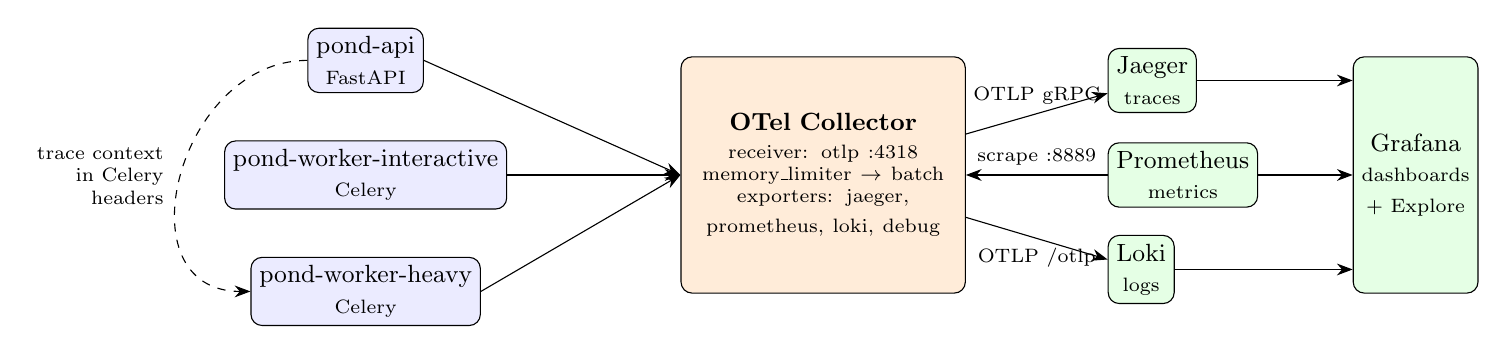
\begin{tikzpicture}[
  box/.style={draw,rounded corners,align=center,font=\small,minimum height=8mm,inner sep=3pt},
  app/.style={box,fill=blue!8}, coll/.style={box,fill=orange!15}, be/.style={box,fill=green!10},
  >={Stealth[length=2mm]}, node distance=6mm and 10mm]
  \node[app] (api) {pond-api\\\scriptsize FastAPI};
  \node[app,below=of api] (wi) {pond-worker-interactive\\\scriptsize Celery};
  \node[app,below=of wi] (wh) {pond-worker-heavy\\\scriptsize Celery};
  \node[coll,right=22mm of wi,minimum height=30mm,text width=34mm] (col)
     {\textbf{OTel Collector}\\[2pt]\scriptsize receiver: otlp :4318\\\scriptsize memory\_limiter $\rightarrow$ batch\\\scriptsize exporters: jaeger,\\\scriptsize prometheus, loki, debug};
  \node[be,right=18mm of col,yshift=12mm] (jae) {Jaeger\\\scriptsize traces};
  \node[be,right=18mm of col] (prom) {Prometheus\\\scriptsize metrics};
  \node[be,right=18mm of col,yshift=-12mm] (loki) {Loki\\\scriptsize logs};
  \node[be,right=12mm of prom,minimum height=30mm] (gr) {Grafana\\\scriptsize dashboards\\\scriptsize + Explore};
  \foreach \n in {api,wi,wh} \draw[->] (\n.east) -- (col.west);
  \draw[->] (col) -- node[above,font=\scriptsize]{OTLP gRPC} (jae);
  \draw[->] (prom) -- node[above,font=\scriptsize]{scrape :8889} (col);
  \draw[->] (col) -- node[below,font=\scriptsize]{OTLP /otlp} (loki);
  \foreach \n in {jae,prom,loki} \draw[->] (\n.east) -- (gr.west |- \n.east);
  \draw[->,dashed] (api.west) to[out=180,in=180,looseness=1.4] node[left,font=\scriptsize,align=right,xshift=-1mm]{trace context\\in Celery\\headers} (wh.west);
\end{tikzpicture}
\caption{Telemetry path. Each process pushes OTLP/HTTP to the collector; the collector fans
signals out to one backend each; Grafana reads all three. Dashed: the trace context travels
with the job through Redis, so the worker's spans join the API's trace.}
\label{fig:arch}
\end{figure}

\subsection{What is instrumented}
Table~\ref{tab:inst} lists every source of telemetry. Most of it is \emph{automatic}: an
instrumentation library patches a framework the app already uses. The domain-specific parts
are \emph{manual}.

\begin{table}[h]
  \caption{Sources of telemetry (\texttt{app/core/telemetry.py})}\label{tab:inst}
  \small
  \begin{tabularx}{\linewidth}{@{}lL@{}}
    \toprule
    Source & What it emits \\
    \midrule
    FastAPI instrumentation & a server span per request (route, method, status); \texttt{http.server.request.duration} histogram \\
    SQLAlchemy instrumentation & a span per SQL statement, with the statement text \\
    Redis instrumentation & a span per Redis command (\texttt{LPUSH}, \texttt{LLEN}, \ldots) \\
    Celery instrumentation & \texttt{apply\_async} (publish) and \texttt{run} (execute) spans; injects and extracts the trace context in message headers \\
    urllib instrumentation & a client span per outbound call: Open-Meteo, NASA POWER, SoilGrids, Nominatim \\
    \textbf{Job span} (manual) & \texttt{job <kind>} around each analysis, with the job id, outcome and key results (\texttt{pond.catchment.area\_ha}) \\
    \textbf{Stage spans} (manual) & one child span per pipeline stage, e.g.\ \texttt{stage: filling sinks (Priority-Flood)} \\
    \textbf{Domain metrics} (manual) & \texttt{pond.job.duration}, \texttt{pond.job.stage.duration} (s), \texttt{pond.jobs.active}, \texttt{pond.catchment.area} (ha), \texttt{pond.design.storage} (m\textsuperscript{3}) \\
    OTLP log handler & every log record at INFO and above, with its trace and span id \\
    \bottomrule
  \end{tabularx}
\end{table}

\subsection{Stage spans without touching the algorithms}
The hydrology engines are pure numpy, and a test (\texttt{tests/test\_layering.py}) fails
the build if a framework is imported into them. Putting \texttt{tracer.start\_span} inside
them would break that rule. Every workflow already records its progress with
\texttt{jobs.update(stage="filling sinks (Priority-Flood)")} for the progress bar in the UI.
\texttt{StageObservingJobs} is a Decorator around the job repository that turns each change
of \texttt{stage} into a span:
\begin{lstlisting}[language=Python]
def update(self, job_id, **fields):
    stages = _stage_spans.get()            # set by job_span() for this job only
    stage = fields.get("stage")
    if stages is not None and isinstance(stage, str):
        if stage in {"done", "failed", "compensated"}:
            stages.close(error=...)        # end the last stage span
        else:
            stages.enter(stage)            # end previous, start + make current the next
    return self._inner.update(job_id, **fields)
\end{lstlisting}
Each stage span is made \emph{current}, so the SQL and HTTP spans emitted during that stage
nest under it. The engines import nothing new, so the layering test still passes.

\subsection{Context propagation and log correlation}
\begin{itemize}
  \item \textbf{Across processes.} The Celery instrumentation writes the W3C
    \texttt{traceparent} into the task message; the worker reads it back, so its spans
    join the API's trace.
  \item \textbf{Across threads.} On the lab deployment, the thread-pool job runner submits
    each job inside \texttt{contextvars.copy\_context()}, which carries the same context
    into the pool thread.
  \item \textbf{Logs.} The OTLP \texttt{LoggingHandler} sits on the root logger. It is
    re-attached after our logging setup and after Celery's, because both replace the
    root handlers. Every exported record carries its trace and span id. The JSON stdout
    formatter adds the same ids:
\end{itemize}
\begin{lstlisting}
{"ts": "2026-10-16T07:19:37+0000", "level": "INFO", "logger": "uvicorn.access",
 "message": "172.21.0.1:61746 - \"GET /api/v1/jobs/ea6f4f0b-... HTTP/1.1\" 200",
 "trace_id": "f99435df7fb3cd30071f41000a09e5be", "span_id": "19522e380ff6f544"}
\end{lstlisting}

\subsection{Tools, libraries and services}
\begin{table}[h]
  \caption{Tools used}\label{tab:tools}
  \small
  \begin{tabularx}{\linewidth}{@{}lL@{}}
    \toprule
    Component & Version and role \\
    \midrule
    \texttt{opentelemetry-sdk}, \texttt{-api} & 1.45.1 --- TracerProvider, MeterProvider, LoggerProvider; batch processors \\
    \texttt{opentelemetry-exporter-otlp-proto-http} & 1.45.1 --- OTLP/HTTP exporters for the three signals \\
    \texttt{opentelemetry-instrumentation-*} & 0.66b1 --- fastapi, sqlalchemy, redis, celery, urllib, logging \\
    OpenTelemetry Collector (contrib) & 0.111.0 --- receiver, processors, four exporters (\texttt{infra/otel/collector.yaml}) \\
    Jaeger all-in-one & 1.62.0 --- trace storage and UI (:16686) \\
    Prometheus & 2.53.0 --- scrapes the collector's metric endpoint \\
    Grafana Loki & 3.2.0 --- log store with a native OTLP endpoint \\
    Grafana & 11.1.0 --- dashboard \emph{Pond --- OpenTelemetry} and Explore; Loki$\leftrightarrow$Jaeger links \\
    \bottomrule
  \end{tabularx}
\end{table}

\textbf{Running it.} \texttt{make up} starts 14 containers, the three new ones being
\texttt{otel-collector}, \texttt{jaeger} and \texttt{loki}. Telemetry is switched on by
\texttt{POND\_OTEL\_ENABLED=true}, which is the Compose default. \texttt{make seed} then
analyses the sample map. \textbf{Verification:} \texttt{tests/test\_telemetry.py} uses
in-memory exporters to assert five things:
\begin{enumerate}
  \item the stage spans are children of the job span;
  \item a failed job marks its stage and the job span as errors;
  \item JSON log lines carry the trace id;
  \item exported logs carry their trace context;
  \item one upload is one trace, from \texttt{POST /api/v1/analyzeContour} down to the
    Priority-Flood stage.
\end{enumerate}
The full suite (226 tests), \texttt{ruff} and \texttt{mypy --strict} pass.

%% =================================================================================
\section{Results: screenshots from the running system}
All screenshots below come from this project running locally under Docker Compose on
16~October~2026. They follow two user actions in the browser:
\begin{enumerate}
  \item analysing the provided sample contour map (\texttt{contours\_1m.kml}, the Khapri
    area of Durg);
  \item clicking the top-ranked site and designing a pond there.
\end{enumerate}

\begin{figure}[h]
  \centering
  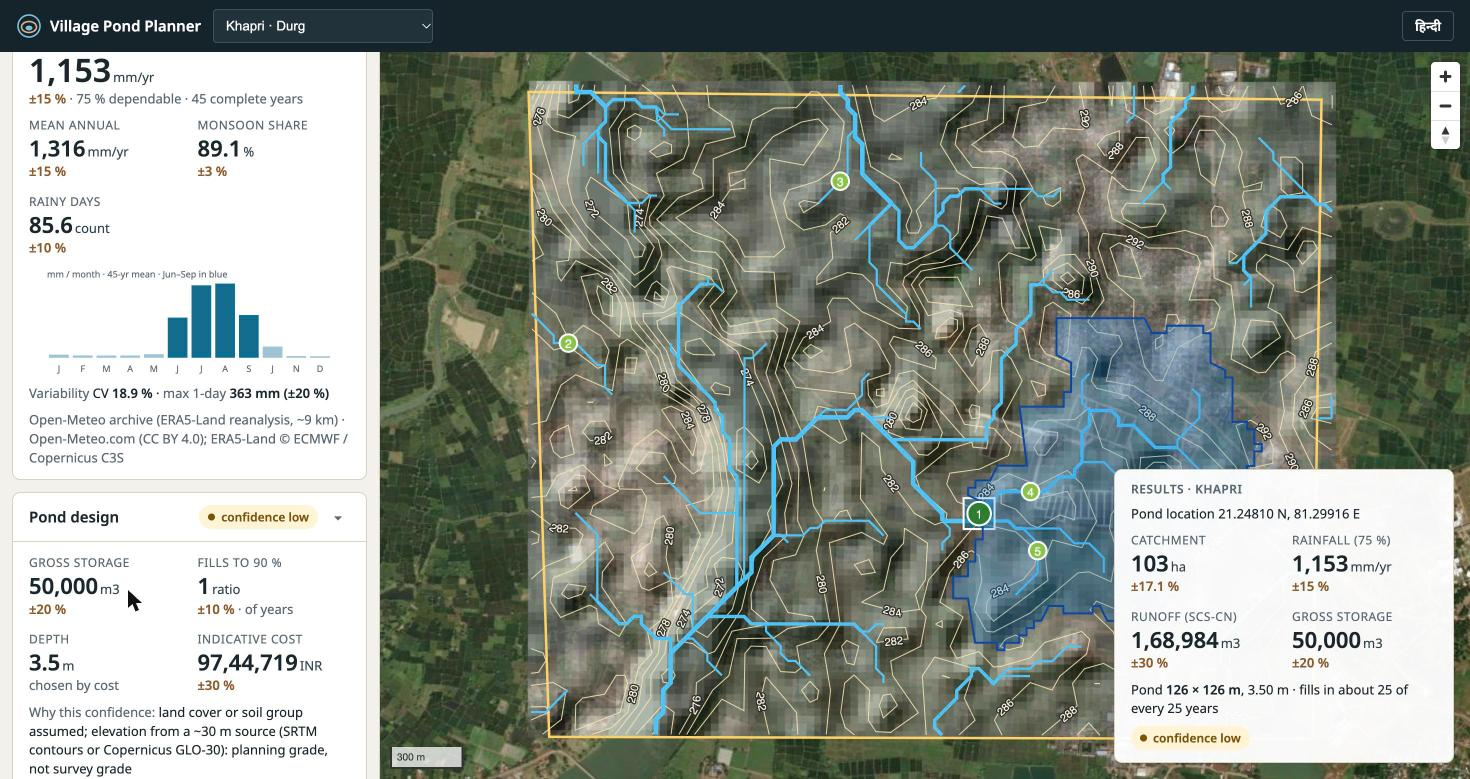
\includegraphics[width=\linewidth]{figures/01-app-result.jpg}
  \caption{The application being observed. Site~\#1 has a 103\,ha catchment (blue). The
  pond design gives 50\,000\,m\textsuperscript{3} and fills in about 25 of 25 years. The
  confidence badge reads ``low'', and Figure~\ref{fig:error} explains why.}
  \label{fig:app}
\end{figure}

\subsection{One trace across three processes}
\begin{figure}[h]
  \centering
  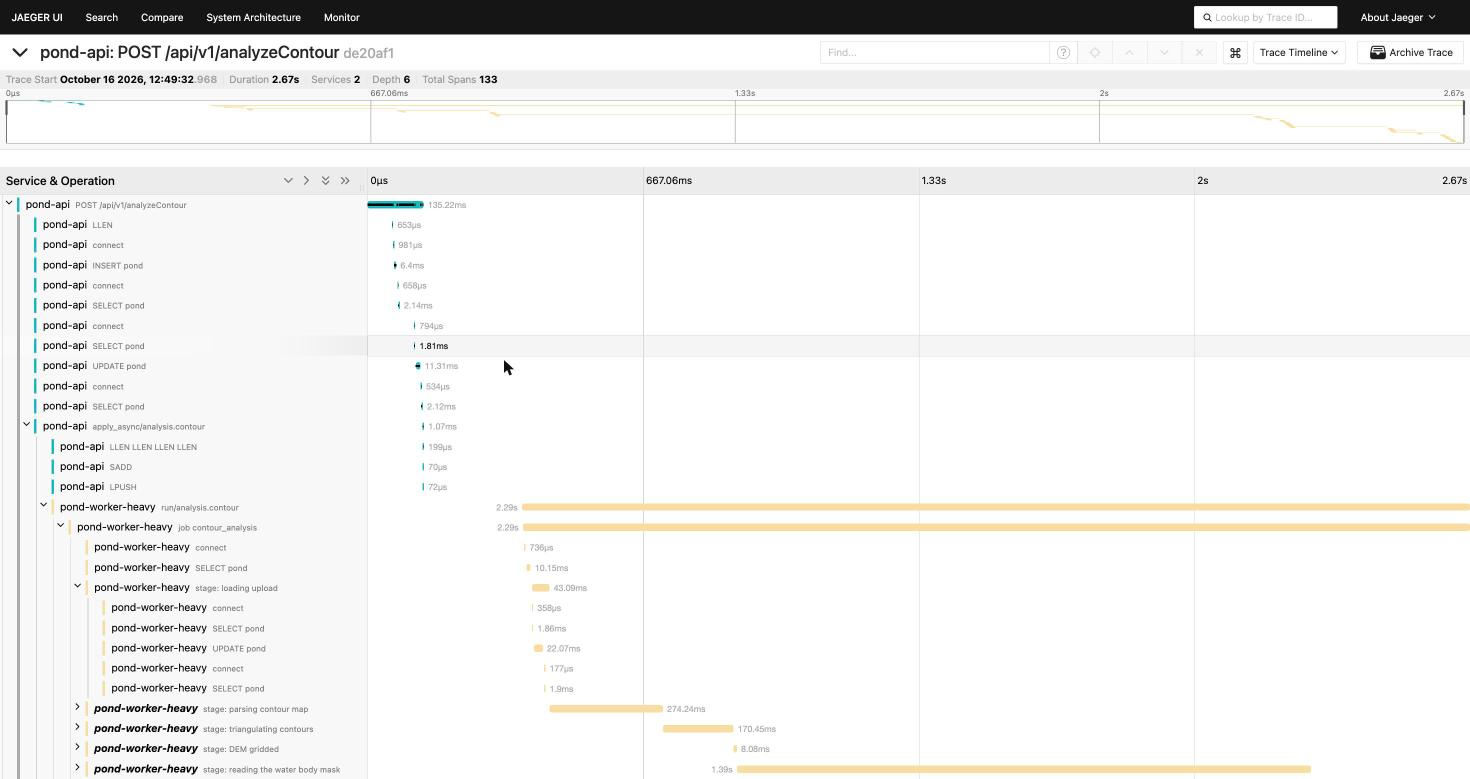
\includegraphics[width=\linewidth]{figures/02-jaeger-trace-api-to-worker.jpg}
  \caption{Jaeger, trace \texttt{de20af1} (133 spans, 2 services, 2.67\,s): one sample-map
  upload.}
  \label{fig:trace}
\end{figure}
Figure~\ref{fig:trace} shows the trace for one upload, top to bottom:
\begin{enumerate}
  \item \textbf{API} (\texttt{pond-api}, teal): the \texttt{POST /api/v1/analyzeContour}
    server span. Under it are the SQL statements that create the job row (\texttt{INSERT
    pond}, \texttt{SELECT pond}) and a Redis \texttt{LLEN}, which is the backpressure
    check on queue depth.
  \item \textbf{Broker:} \texttt{apply\_async/analysis.contour} with its \texttt{LPUSH},
    which puts the job on the Redis queue.
  \item \textbf{Worker} (\texttt{pond-worker-heavy}, yellow): \texttt{run/analysis.contour}
    and our \texttt{job contour\_analysis} span.
\end{enumerate}
The worker spans are in the \emph{same trace} as the HTTP request although they ran in
another container: the context crossed Redis in the message headers. The gap between the
API returning (135\,ms) and the worker starting is the queueing delay, visible directly.
Expanding \texttt{stage: loading upload} shows its SQL nested under it.

\subsection{The algorithm as a waterfall}
\begin{figure}[h]
  \centering
  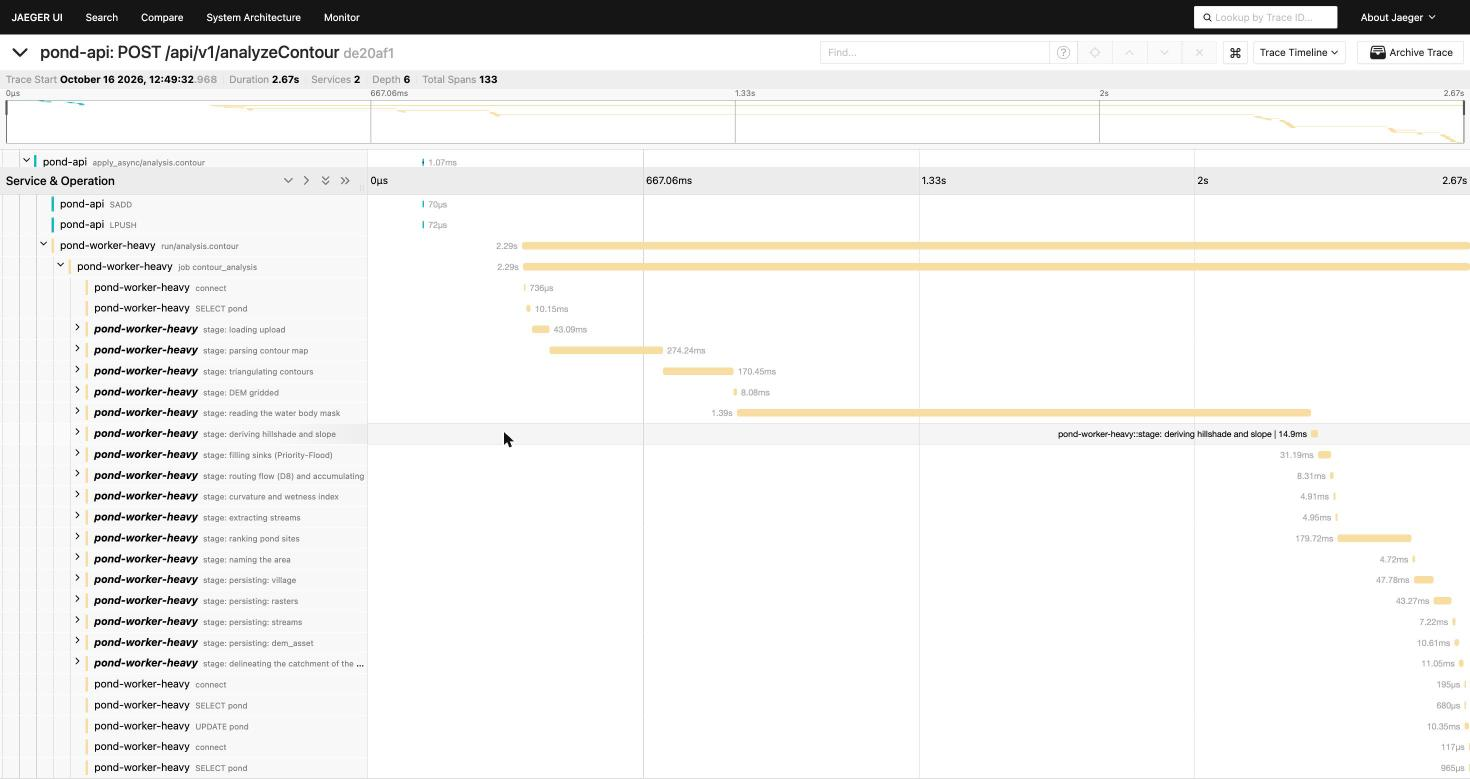
\includegraphics[width=\linewidth]{figures/03-jaeger-algorithm-stages.jpg}
  \caption{The same trace, scrolled to the worker: one span per pipeline stage, in
  execution order.}
  \label{fig:stages}
\end{figure}
Figure~\ref{fig:stages} reads as the methodology section of the main report:
\begin{itemize}
  \item parsing the KML (274\,ms) and triangulating the contours (170\,ms);
  \item reading the water-body mask (1.39\,s);
  \item filling sinks with Priority-Flood (31\,ms) and D8 flow routing with accumulation
    (8\,ms);
  \item extracting streams (5\,ms) and ranking pond sites (180\,ms);
  \item persisting (about 110\,ms) and delineating the top site's catchment (11\,ms).
\end{itemize}

\textbf{What this told us.} The examined algorithms are not the bottleneck. Priority-Flood,
D8 and catchment delineation together take about 50\,ms. The single largest stage is
\emph{reading the water body mask}, a window read of a Copernicus GLO-30 file on AWS S3. It
took 1.39\,s of 2.67\,s here (52\,\%) and 1.85\,s of 2.66\,s on the first run (70\,\%). The
right optimisation is therefore to cache the mask per tile, not to speed up the hydrology.
Without stage spans we would have guessed the opposite.

\subsection{Debugging a degraded result}
\begin{figure}[h]
  \centering
  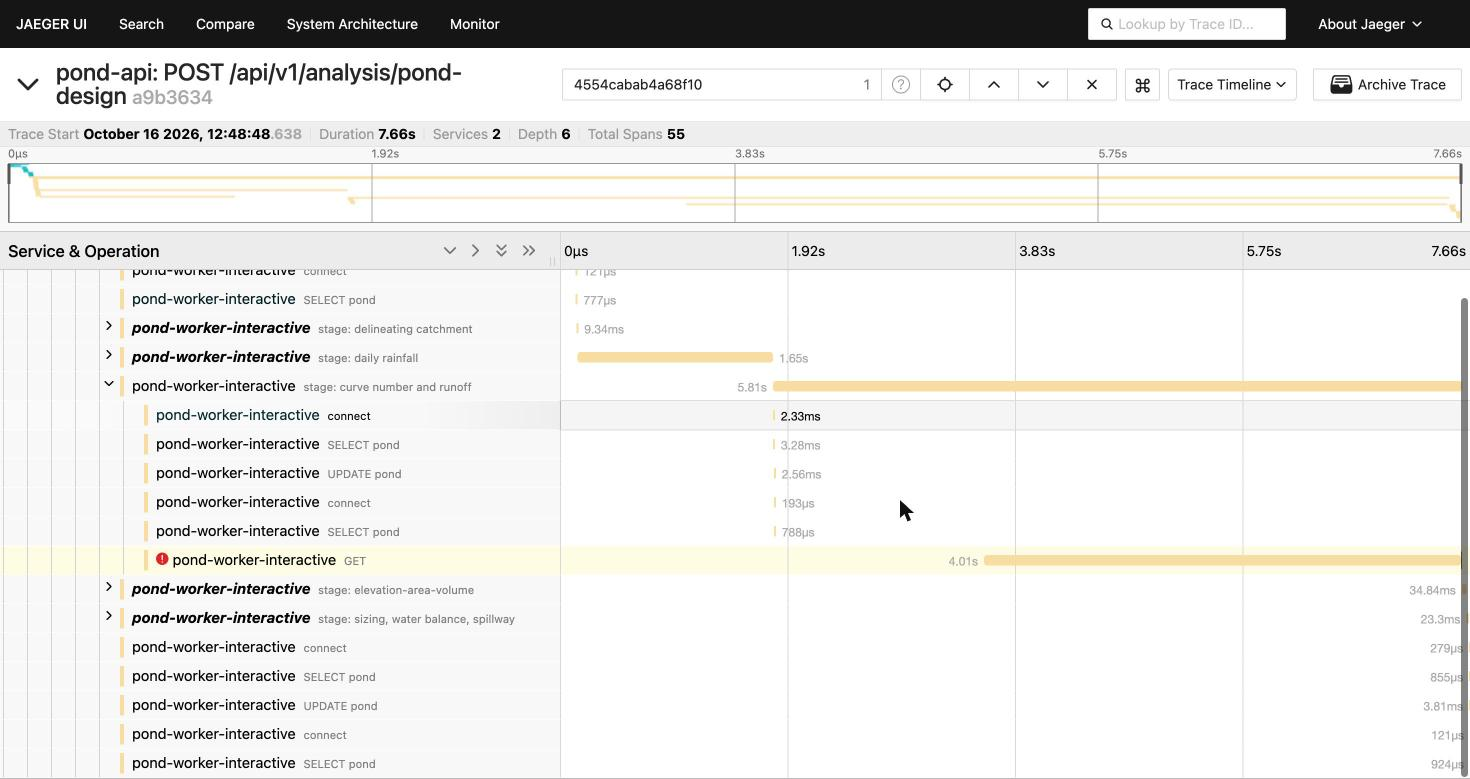
\includegraphics[width=\linewidth]{figures/04-jaeger-pond-design-error.jpg}
  \caption{Jaeger, trace \texttt{a9b3634}: the pond design (7.66\,s). The
  \texttt{curve number and runoff} stage holds a failed outbound \texttt{GET} (red marker)
  that took 4.01\,s.}
  \label{fig:error}
\end{figure}
The pond design in Figure~\ref{fig:app} was labelled ``confidence low: land cover or soil
group assumed''. Its trace (Figure~\ref{fig:error}) shows the breakdown:
\begin{itemize}
  \item delineating the catchment: 9\,ms;
  \item fetching 45 years of daily rainfall: 1.65\,s, of which 1.03\,s is the Open-Meteo
    \texttt{GET};
  \item the curve-number stage: 5.81\,s, of which 4.01\,s is one failed \texttt{GET},
    marked as an error.
\end{itemize}
The failing span's attributes, read from Jaeger, name the call and the reason:
\begin{lstlisting}
url.full            = https://rest.isric.org/soilgrids/v2.0/properties/query?lon=81.2992&lat=21.2481&...
error.type          = URLError
otel.status_code    = ERROR
otel.status_description = URLError: <urlopen error [Errno -5] No address associated with hostname>
event: exception    (exception.type = urllib.error.URLError, with stack trace)
\end{lstlisting}
So the ``low confidence'' was not a modelling problem. The soil database's \emph{hostname
did not resolve} for 4\,s, the provider fell back to a stated default soil group, and the
design said so. A later lookup from the same container resolved normally, so this was the
campus network's intermittent DNS, the same fault that reset Docker Hub pulls during setup.
The trace also shows the cost: 4\,s of a 7.7\,s request was spent waiting on a name lookup,
which argues for a shorter DNS/connect timeout on that provider.

\begin{figure}[h]
  \centering
  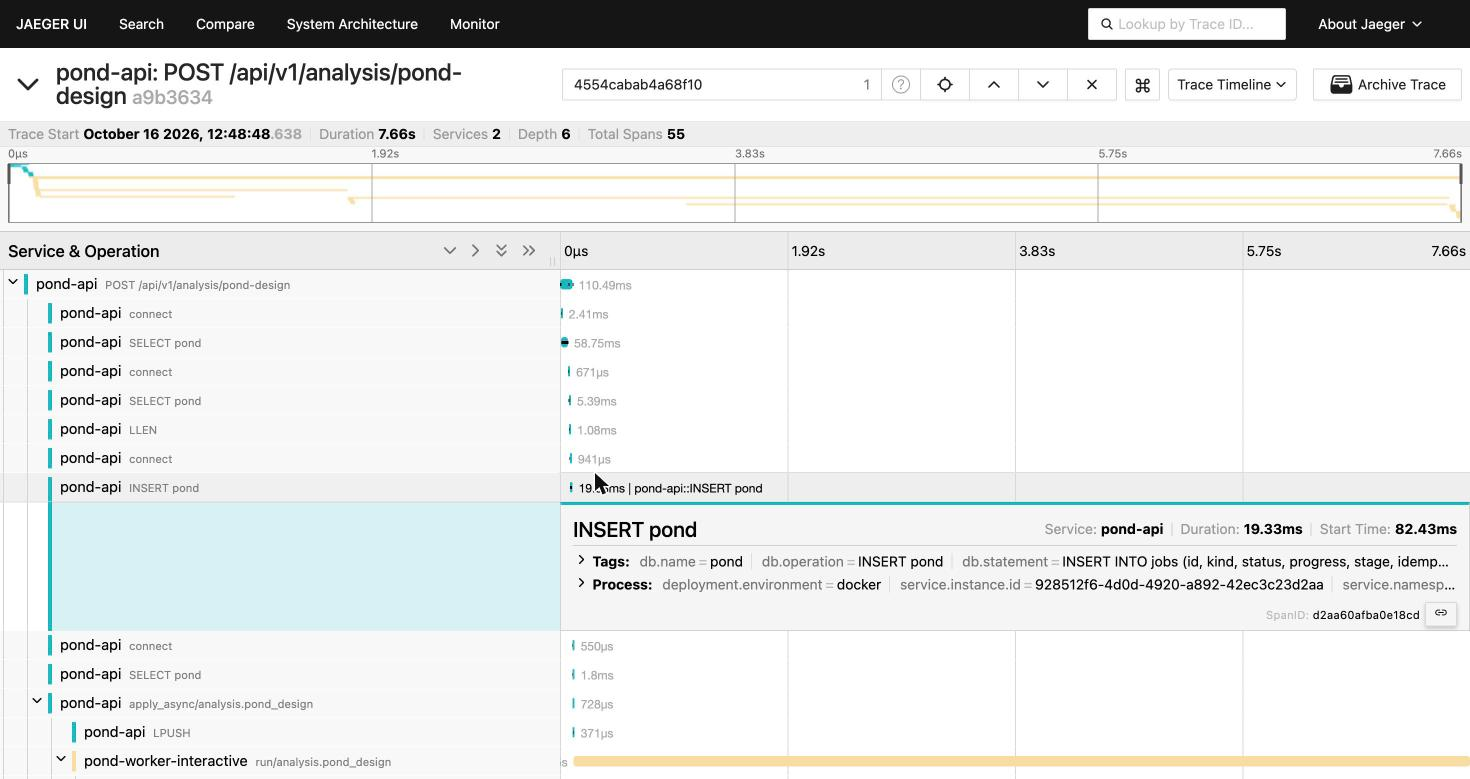
\includegraphics[width=\linewidth]{figures/05-jaeger-sql-span-detail.jpg}
  \caption{Span detail for an automatically instrumented SQL statement (\texttt{INSERT
  pond}, 19\,ms). The SQLAlchemy instrumentation records \texttt{db.system},
  \texttt{db.name} and the statement; the Process block lists the Resource attributes
  that identify the container.}
  \label{fig:sql}
\end{figure}

\subsection{Logs, correlated to the trace}
\begin{figure}[h]
  \centering
  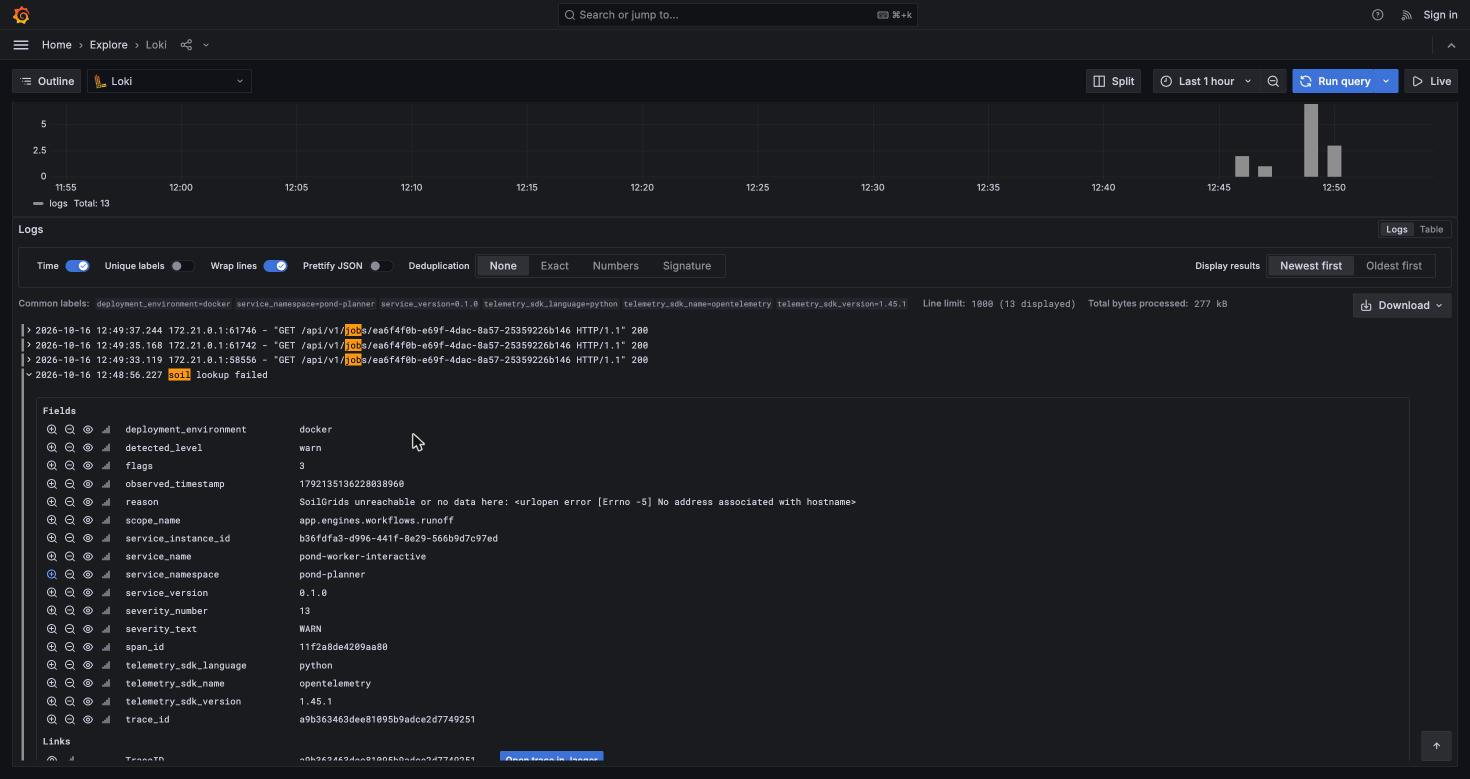
\includegraphics[width=\linewidth]{figures/07-loki-log-with-trace-id.jpg}
  \caption{Grafana Explore over Loki: the worker's \texttt{WARN soil lookup failed} record,
  exported over OTLP. It carries the reason, its service, \texttt{span\_id} and
  \texttt{trace\_id = a9b363463dee\ldots}; the \emph{Open trace in Jaeger} link goes to
  the trace in Figure~\ref{fig:error}.}
  \label{fig:logs}
\end{figure}
Figure~\ref{fig:logs} is the same incident seen from the log side. The warning has the
\emph{same trace id} as the trace in Figure~\ref{fig:error}. That is the practical value
of correlation: starting from either a slow request or an error message, one click reaches
the other half of the evidence. Grepping timestamps across three containers is no longer
needed.

\subsection{Metrics}
\begin{figure}[h]
  \centering
  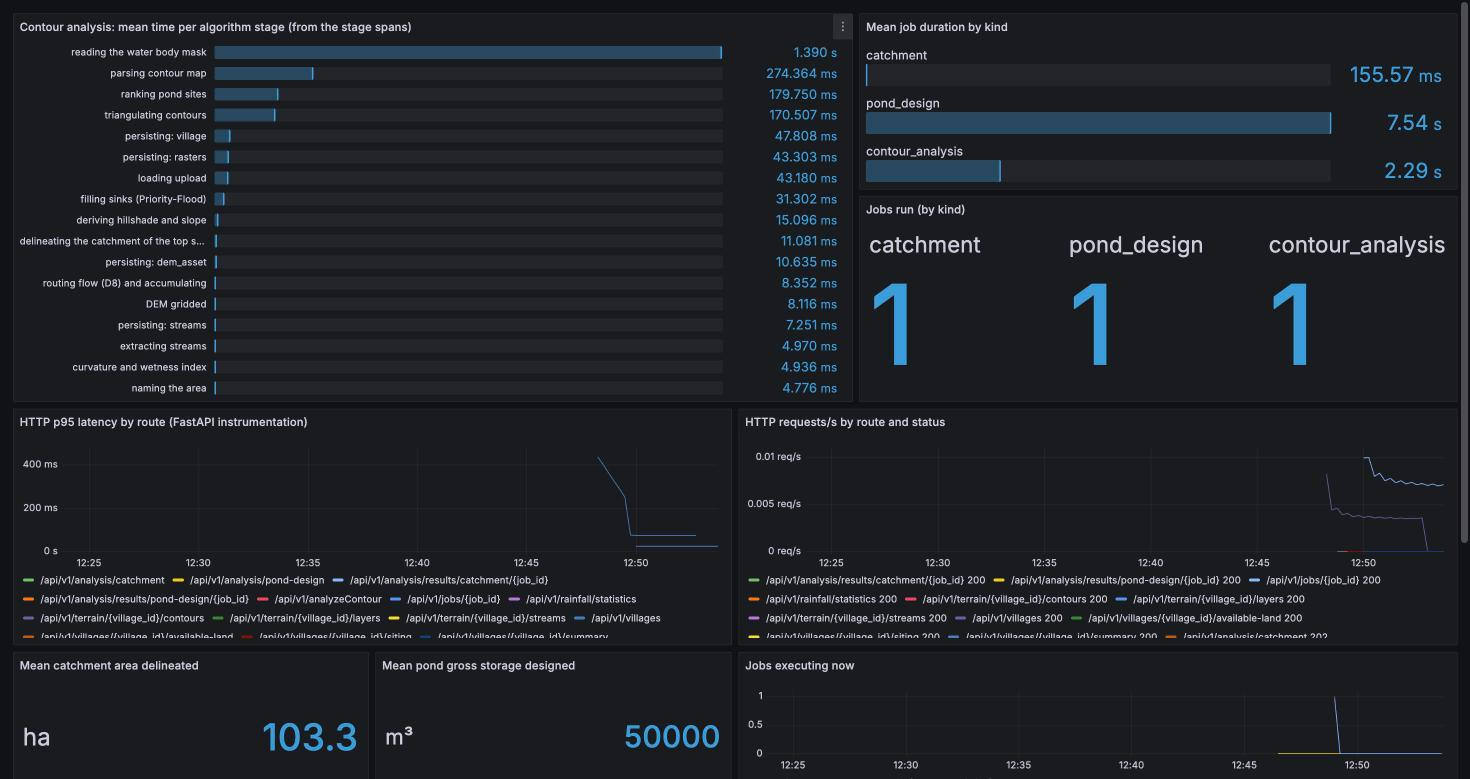
\includegraphics[width=\linewidth]{figures/06-grafana-otel-metrics.jpg}
  \caption{Grafana dashboard \emph{Pond --- OpenTelemetry}, from the OTel metrics in
  Prometheus.}
  \label{fig:metrics}
\end{figure}
Figure~\ref{fig:metrics} has six parts:
\begin{itemize}
  \item \textbf{Top left:} mean time per pipeline stage, sorted. This is the
    \texttt{pond.job.stage.duration} histogram recorded as each stage span ends; the same
    finding as Figure~\ref{fig:stages}, but aggregated over every run.
  \item \textbf{Top right:} mean job duration by kind (catchment 156\,ms, contour analysis
    2.29\,s, pond design 7.54\,s) and job counts.
  \item \textbf{Middle:} HTTP p95 latency and request rate per route, from the FastAPI
    instrumentation.
  \item \textbf{Bottom:} the domain metrics. The mean catchment delineated is 103.3\,ha,
    the mean designed storage is 50\,000\,m\textsuperscript{3}, and a gauge counts jobs
    executing now.
\end{itemize}

Traces explain \emph{one} request; metrics show the \emph{trend}. For example, a regression
in ranking time would show here before anyone opened a trace.

Behind the screenshots, the collector's \texttt{debug} exporter proves that all three
pipelines are flowing (\texttt{docker logs pond-planner-otel-collector-1}):
\begin{lstlisting}
info  MetricsExporter {"data_type": "metrics", "resource metrics": 2, "metrics": 16, "data points": 49}
info  LogsExporter    {"data_type": "logs", "resource logs": 1, "log records": 2}
info  TracesExporter  {"data_type": "traces", "resource spans": 2, "spans": 11}
\end{lstlisting}

%% =================================================================================
\section{Understanding: what OpenTelemetry gives this system}
\begin{description}
  \item[Monitoring.] The dashboard answers ``is it healthy and how fast'' continuously:
    request rates and p95 latency per route, job durations by kind, jobs in flight, and the
    domain outputs themselves. A sudden fall in mean catchment area would flag a broken DEM
    source, not just a slow one.
  \item[Debugging.] A trace turns ``the design says low confidence'' into ``SoilGrids DNS
    failed after 4\,s in this stage of this job''. The error span carries the exception and
    stack trace, and the correlated log says what the code decided to do about it.
  \item[Performance analysis.] Stage spans showed that network I/O, not hydrology, dominates
    the pipeline. They also show the queueing delay between API and worker, which is the
    number to watch when the bulkhead pools are resized.
  \item[Understanding the architecture.] The trace \emph{is} the sequence diagram of the
    asynchronous job design (ADR~0008): API, then Redis, then worker, then stages. It is
    generated from the running code, not drawn by hand, so it cannot go out of date.
\end{description}

\textbf{Design choices and their reasons.}
\begin{itemize}
  \item \textbf{A collector rather than direct export.} It keeps backends out of the code,
    and it batches and limits memory in one place.
  \item \textbf{Explicit SDK setup rather than the zero-code agent.} The agent cannot see
    pipeline stages, and about 80 lines of setup can be explained line by line.
  \item \textbf{Batch processors.} Spans are exported on a background thread, so a request
    never waits on the collector. The cost is a few seconds before a trace is visible.
  \item \textbf{OTel metrics beside \texttt{prometheus\_client}.} The OTel metrics run
    alongside the existing P6 metrics rather than replacing them, because the backpressure
    logic and the P6 dashboard depend on the old ones.
\end{itemize}
The full record is ADR~0022 in the repository.

\textbf{Limits, stated.}
\begin{itemize}
  \item Reads of the Copernicus DEM go through GDAL's C library (libcurl), which Python
    instrumentation cannot see. They appear as stage time, not as HTTP spans.
  \item The Celery worker writes stdout in Celery's own format, so trace ids appear in its
    \emph{exported} logs, not in its console.
  \item The lab VMs cannot run Docker, so the deployed replicas keep telemetry off by
    default.
  \item Sampling is 100\,\%, which is right for a demo and wrong for production volume,
    where a tail-sampling processor in the collector would keep only slow or failed traces.
\end{itemize}

\textbf{Repository.} \url{\repourl} --- \texttt{app/core/telemetry.py},
\texttt{infra/otel/collector.yaml}, \texttt{infra/grafana/dashboards/pond-otel.json},
\texttt{tests/test\_telemetry.py}, \texttt{docs/adr/0022-opentelemetry.md}.

\textbf{AI tool use.} Claude (Anthropic) was used as a coding assistant for the
instrumentation, the configuration and this report. Every design decision above was
reviewed and can be explained by the author.

\end{document}
